\documentclass[11pt,a4paper]{article}
\usepackage[margin=2.5cm]{geometry}
\usepackage{amsmath,amssymb,amsthm}
\usepackage{graphicx}
\usepackage{booktabs}
\usepackage{hyperref}
\usepackage{xcolor}
\emergencystretch=2em
\hypersetup{colorlinks=true,linkcolor=blue!50!black,citecolor=blue!50!black,urlcolor=blue!50!black}

\newtheorem{definition}{Definition}
\newtheorem{conjecture}{Conjecture}
\newtheorem{proposition}{Proposition}
\theoremstyle{remark}
\newtheorem{remark}{Remark}

\title{Prime Clustering in Polynomial $Q(n) = n^q - (n-1)^q$:\\
Quadruplet Distribution, Riemann Zero Correlation,\\
and a 200{,}000-Digit $Q_{47}$ Probable Prime\\[4pt]
\large An Empirical Study Based on 18 Million Verified Primes --- Version 2}
\author{Ruqing Chen\\
GUT Geoservice Inc., Montreal, Canada\\
\texttt{ruqing@hotmail.com}}
\date{October 2026 (v2; v1: January 2026)\\[2pt]
\small DOI: \href{https://doi.org/10.5281/zenodo.23517573}{10.5281/zenodo.23517573}}

\begin{document}
\maketitle

\begin{abstract}
We present a comprehensive computational study of prime-generating polynomials $Q(n) = n^q - (n-1)^q$ for seven prime exponents $q = 37$, $41$, $43$, $47$, $53$, $61$, $71$. Analyzing 18,356,706 verified primes in the range $n \in [1, 2\times10^9]$, we discover 15 quadruplet systems for $Q_{47}$, compared to at most 2 for all other polynomials. A correlation ($r = 0.994$) emerges between quadruplet positions and Riemann zeta zeros under the scaling $n^{1/\alpha}$; in this version we calibrate it against a null model of randomly placed quadruplets and find that it is only marginally significant ($P \approx 0.05$). We propose the Subgroup Interference Hypothesis: the interference potential $I(q) = d(q-1) - 2$ determines clustering stability by minimizing the topological complexity of the sieve space.

New in version 2, we extend the $Q_{47}$ data set by more than four hundred orders of magnitude in $n$: a sieve-and-PRP search in a window of $1.5\times10^5$ consecutive values of $n \approx 5.86\times10^{4347}$ found
\[
Q_{47}(n^\ast),\qquad n^\ast = 586135293385\cdot 10^{4336} + 1647,
\]
a probable prime with exactly 200,000 decimal digits (664,383 bits), passing Fermat tests to bases 3, 5, 7 and 11. We believe it is the largest known value of $Q_{47}$ that is a probable prime. The discovery rate agrees with the Bateman--Horn prediction.
\end{abstract}

\noindent\textbf{Keywords:} prime-generating polynomials, prime constellations, safe primes, Riemann zeta zeros, Bateman--Horn conjecture, subgroup lattice, probable primes, PFGW

\section*{Changes in Version 2}
\begin{itemize}
\item \textbf{New Section~\ref{sec:prp}}: a 200,000-digit probable prime $Q_{47}(n^\ast)$, the sieve used to find it, verification records, comparison with Bateman--Horn, and the status of a primality proof.
\item \textbf{Correction (Section~\ref{sec:lattice}, Figure~\ref{fig:lattice})}: the subgroup lattice of $\mathbb{Z}_{47}^\ast$ is a diamond $\{1\}\subset H_2, H_{23}\subset\mathbb{Z}_{47}^\ast$, not a chain; $H_2\not\subset H_{23}$ because $2\nmid 23$. The value $I(47)=2$ is unchanged.
\item \textbf{Calibration (Remark~\ref{rem:null})}: a null-model test of the Riemann-zero correlation of Section~\ref{sec:riemann}.
\end{itemize}

\section{Introduction}
The Bateman--Horn conjecture~\cite{BH} provides a general framework for predicting prime densities in polynomial sequences. For a polynomial $f(x)$ of degree $d$, the asymptotic prime count is
\begin{equation}
\pi_f(N) \sim \frac{C}{d}\cdot\frac{N}{\ln N},
\end{equation}
where $C$ is a product of local densities. In this paper, we investigate the family of polynomials
\begin{equation}
Q(n) = n^q - (n-1)^q,
\end{equation}
where $q$ is a prime exponent. For $q=3$ this is $3n^2-3n+1$, whose prime values are the classical cuban primes; the family studied here is its higher-degree analogue. We focus on the phenomenon of prime constellations: consecutive integers $n, n+1, \dots, n+k-1$ that all produce prime $Q$-values, forming doublets ($k = 2$), triplets ($k = 3$), and quadruplets ($k = 4$).

Our central finding concerns $Q_{47}$, where $q = 47$ is a safe prime:
\begin{equation}
47 = 2\times23 + 1 \qquad (\text{with } 23 \text{ also prime}).
\end{equation}
This unique arithmetic property among our seven test polynomials correlates with remarkable structural stability, enabling the formation of 15 quadruplet systems up to $n = 2\times10^9$.

\section{Data and Methods}
\subsection{Dataset Construction}
We performed exhaustive primality testing on seven polynomial families, with exponents $q = 37$, $41$, $43$, $47$, $53$, $61$ and $71$. For the comparative analysis (Section~\ref{sec:seven}), all polynomials were evaluated over $n \in [1, 10^8]$. For $Q_{47}$, we extended the search to $n \in [1, 2\times10^9]$, yielding
\begin{equation}
\text{Total verified primes: } 18{,}356{,}706.
\end{equation}
Primality was confirmed using Miller--Rabin tests with deterministic witness sets~\cite{Miller}. The large-$n$ search of Section~\ref{sec:prp} uses a different method, described there.

\subsection{Statistical Metrics}
\begin{definition}[Triplet Surplus]
The triplet surplus $S_3$ measures the percentage deviation of observed triplet count from Poisson expectation:
\begin{equation}
S_3 = \frac{O - E}{E}\times 100\%,
\end{equation}
where $O$ is the observed count and $E$ is the expected count under random distribution.
\end{definition}

\begin{definition}[Interference Potential]
The interference potential $I(q)$ quantifies the complexity of the subgroup lattice $\mathcal{L}(\mathbb{Z}_q^\ast)$:
\begin{equation}
I(q) = d(q-1) - 2,
\end{equation}
where $d(n)$ denotes the divisor function. This measures the number of non-trivial subgroups, excluding $\{1\}$ and the full group $\mathbb{Z}_q^\ast$.
\end{definition}

\section{Seven-Polynomial Comparison}\label{sec:seven}
Table~\ref{tab:seven} summarizes the clustering statistics for all seven polynomials in the range $n \in [1, 10^8]$, with extended quadruplet census up to $n = 2\times10^9$.

\begin{table}[h]
\centering
\caption{Clustering statistics with extended-range quadruplet census.}\label{tab:seven}
\begin{tabular}{lccccrc}
\toprule
$Q_q$ & Safe? & $q-1$ & $d(q-1)$ & $I(q)$ & $S_3$ & 4-lets ($n<2\times10^9$)\\
\midrule
$Q_{37}$ & No & $2^2\cdot3^2$ & 9 & 7 & $+20.4\%$ & 2 (decay)\\
$Q_{41}$ & No & $2^3\cdot5$ & 8 & 6 & $+48.8\%$ & 0\\
$Q_{43}$ & No & $2\cdot3\cdot7$ & 8 & 6 & $+15.3\%$ & 1 (decay)\\
$\mathbf{Q_{47}}$ & \textbf{Yes} & $\mathbf{2\cdot23}$ & \textbf{4} & \textbf{2} & $\mathbf{+35.0\%}$ & \textbf{15 (growth)}\\
$Q_{53}$ & No & $2^2\cdot13$ & 6 & 4 & $+30.7\%$ & 0\\
$Q_{61}$ & No & $2^2\cdot3\cdot5$ & 12 & 10 & $-16.7\%$ & 0\\
$Q_{71}$ & No & $2\cdot5\cdot7$ & 8 & 6 & $+20.5\%$ & 0\\
\bottomrule
\end{tabular}
\end{table}

\begin{figure}[h]
\centering
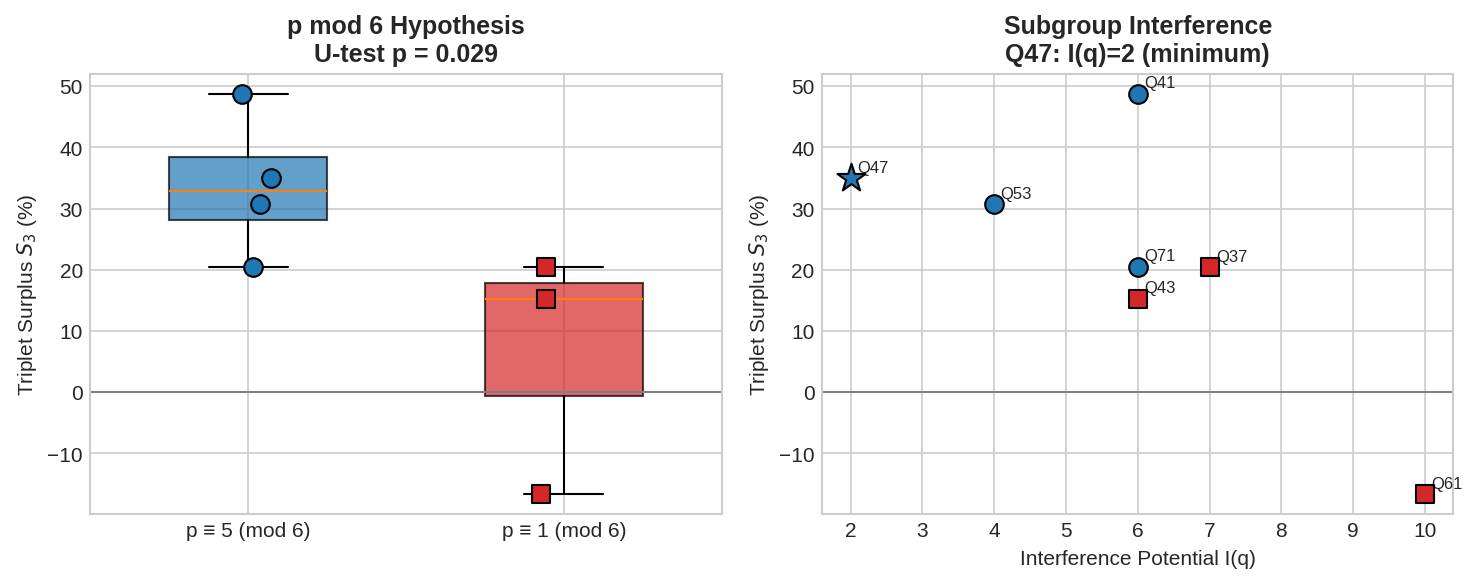
\includegraphics[width=\textwidth]{fig1_surplus.png}
\caption{Triplet surplus $S_3$ distribution by residue class $p \bmod 6$ (left) and interference potential $I(q)$ versus triplet surplus (right). $Q_{47}$ (highlighted) shows moderate $S_3$ with minimal $I(q) = 2$.}
\end{figure}

\noindent\textbf{Key Observations:}
\begin{itemize}
\item $Q_{41}$ exhibits the highest triplet surplus ($+48.8\%$) but produces zero quadruplets, indicating stochastic rather than structural clustering.
\item $Q_{61}$ with maximum $I(q) = 10$ shows negative surplus ($-16.7\%$), demonstrating subgroup-induced suppression.
\item $Q_{47}$ is the only polynomial showing quadruplet growth with extended range.
\end{itemize}

\subsection{Subgroup Lattice Structure}\label{sec:lattice}
For the safe prime $q = 47 = 2\times23 + 1$, the multiplicative group $\mathbb{Z}_{47}^\ast \cong C_{46}$ is cyclic, so its subgroups correspond to the divisors $1, 2, 23, 46$ of $46$, with $H_d\subseteq H_{d'}$ if and only if $d\mid d'$. The lattice is therefore the minimal non-trivial one, a single diamond:
\begin{equation}
\{1\} \subset H_2,\ H_{23} \subset \mathbb{Z}_{47}^\ast, \qquad H_2\cap H_{23}=\{1\},\quad H_2H_{23}=\mathbb{Z}_{47}^\ast .
\end{equation}
(Version 1 wrote this as a chain $\{1\}\subset H_2\subset H_{23}\subset\mathbb{Z}_{47}^\ast$; this is incorrect since $2\nmid 23$.) For any odd prime $q$, $2\mid q-1$ forces $d(q-1)\ge 4$ once $q-1$ has an odd prime factor, so $I(q)=2$ is attained exactly when $q-1=2r$ with $r$ an odd prime, i.e.\ when $q$ is a safe prime. In contrast, $Q_{41}$ ($40 = 2^3\times5$) has an eight-element lattice with multiple chains between $\{1\}$ and the full group.

\begin{figure}[h]
\centering
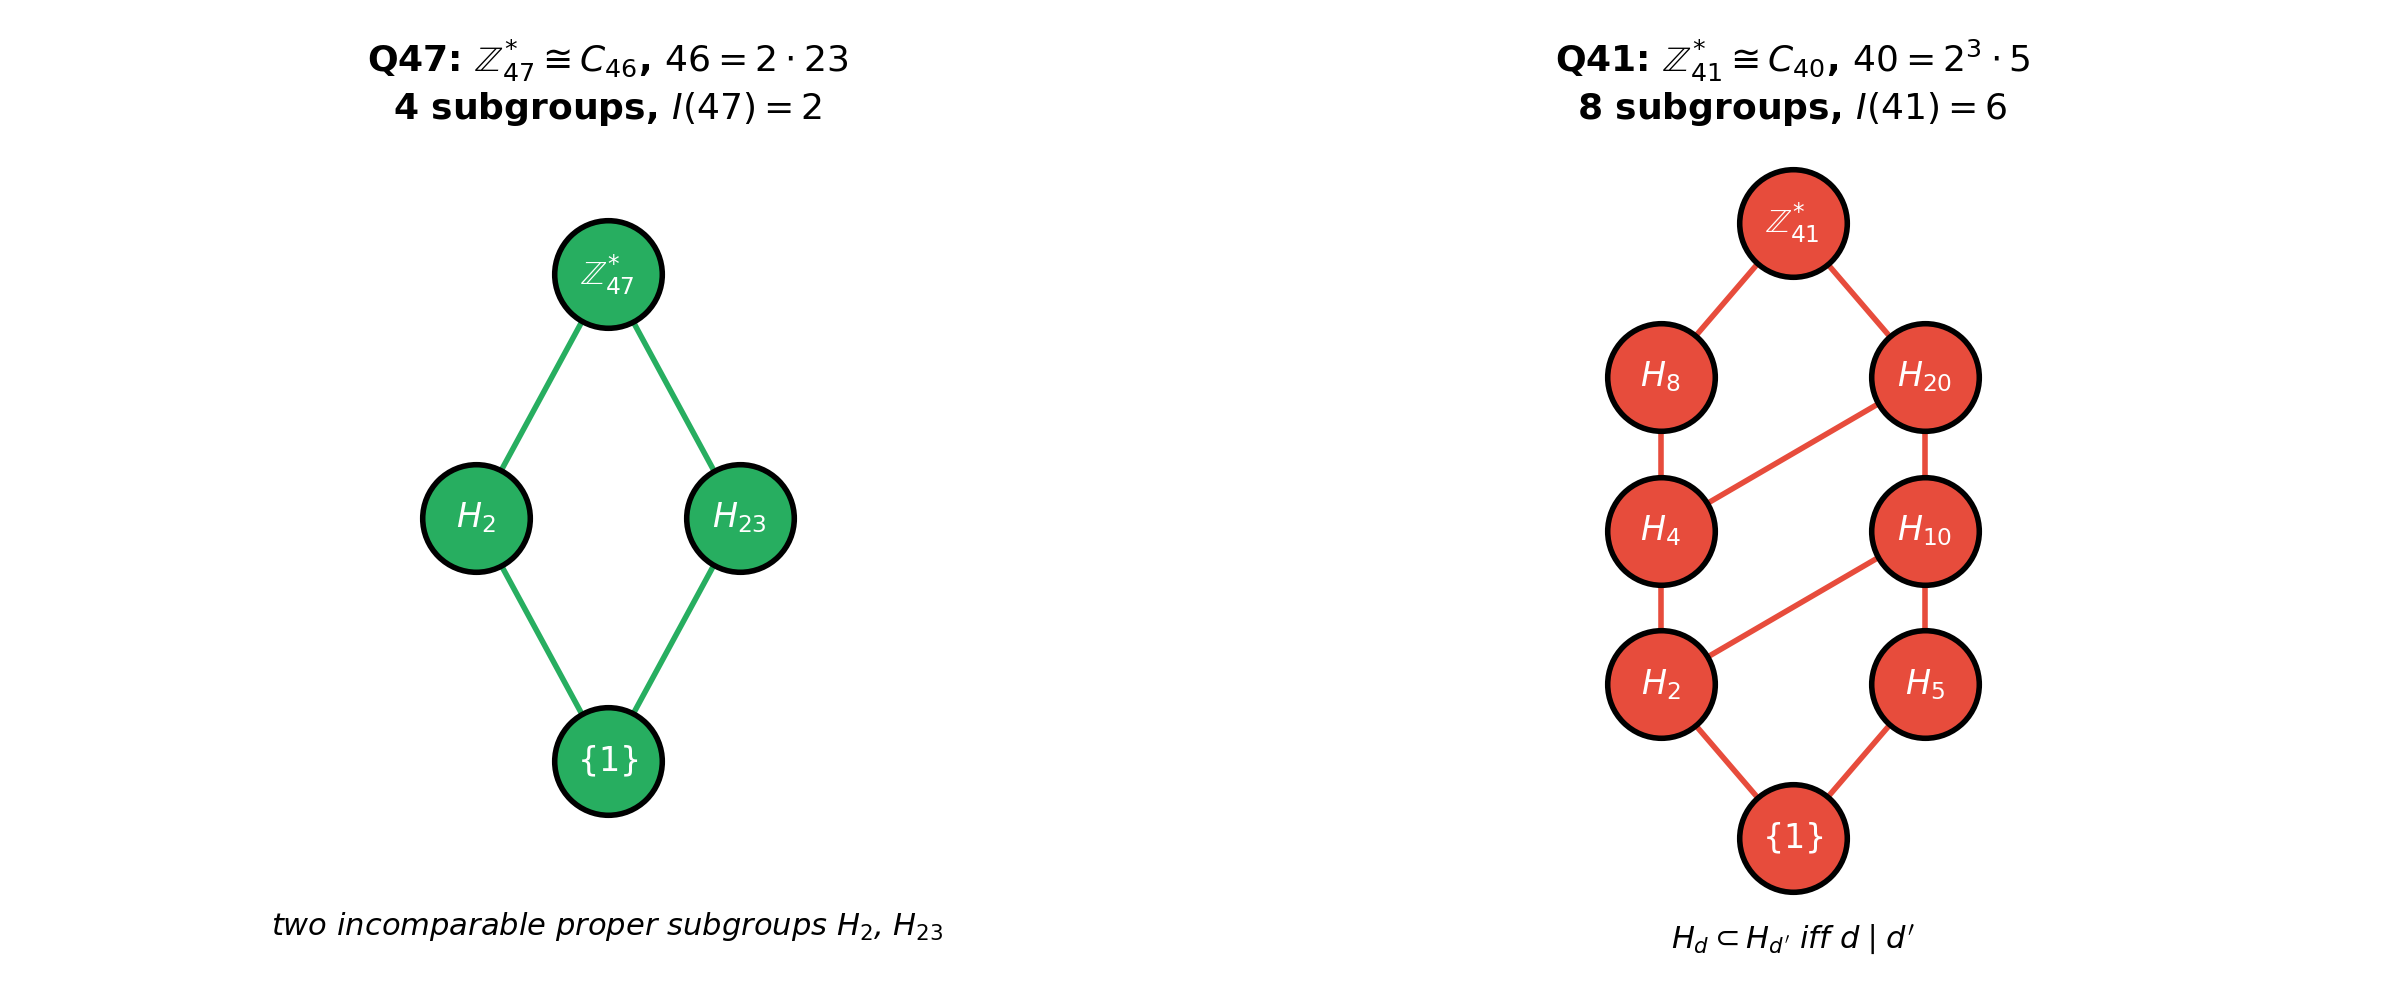
\includegraphics[width=\textwidth]{fig2_lattice_v2.png}
\caption{Subgroup lattice structure (corrected in v2). Left: $\mathbb{Z}_{47}^\ast$ has exactly two proper non-trivial subgroups, $H_2$ and $H_{23}$, which are incomparable, giving $I(47) = 2$. Right: $\mathbb{Z}_{41}^\ast$ has six, giving $I(41) = 6$. Edges join $H_d \subset H_{d'}$ with $d'/d$ prime.}\label{fig:lattice}
\end{figure}

\section{$Q_{47}$ Quadruplet Census}
In the extended range $n \in [1, 2\times10^9]$, we identified 15 quadruplet systems for $Q_{47}$. Table~\ref{tab:quad} provides the complete, verified coordinate list.

\begin{table}[h]
\centering
\caption{Complete coordinate list of $Q_{47}$ quadruplet systems.}\label{tab:quad}
\begin{tabular}{rrr@{\hspace{2.5em}}rrr}
\toprule
$k$ & Starting position $n$ & Range & $k$ & Starting position $n$ & Range\\
\midrule
1 & 23,159,557 & $0.02\times10^9$ & 9 & 987,980,498 & $0.99\times10^9$\\
2 & 117,309,848 & $0.12\times10^9$ & 10 & 1,163,461,515 & $1.16\times10^9$\\
3 & 136,584,738 & $0.14\times10^9$ & 11 & 1,370,439,187 & $1.37\times10^9$\\
4 & 218,787,064 & $0.22\times10^9$ & 12 & 1,643,105,964 & $1.64\times10^9$\\
5 & 411,784,485 & $0.41\times10^9$ & 13 & 1,691,581,855 & $1.69\times10^9$\\
6 & 423,600,750 & $0.42\times10^9$ & 14 & 1,975,860,550 & $1.98\times10^9$\\
7 & 523,331,634 & $0.52\times10^9$ & 15 & 1,996,430,175 & $2.00\times10^9$\\
8 & 640,399,031 & $0.64\times10^9$ & & & \\
\bottomrule
\end{tabular}
\end{table}

\begin{figure}[h]
\centering
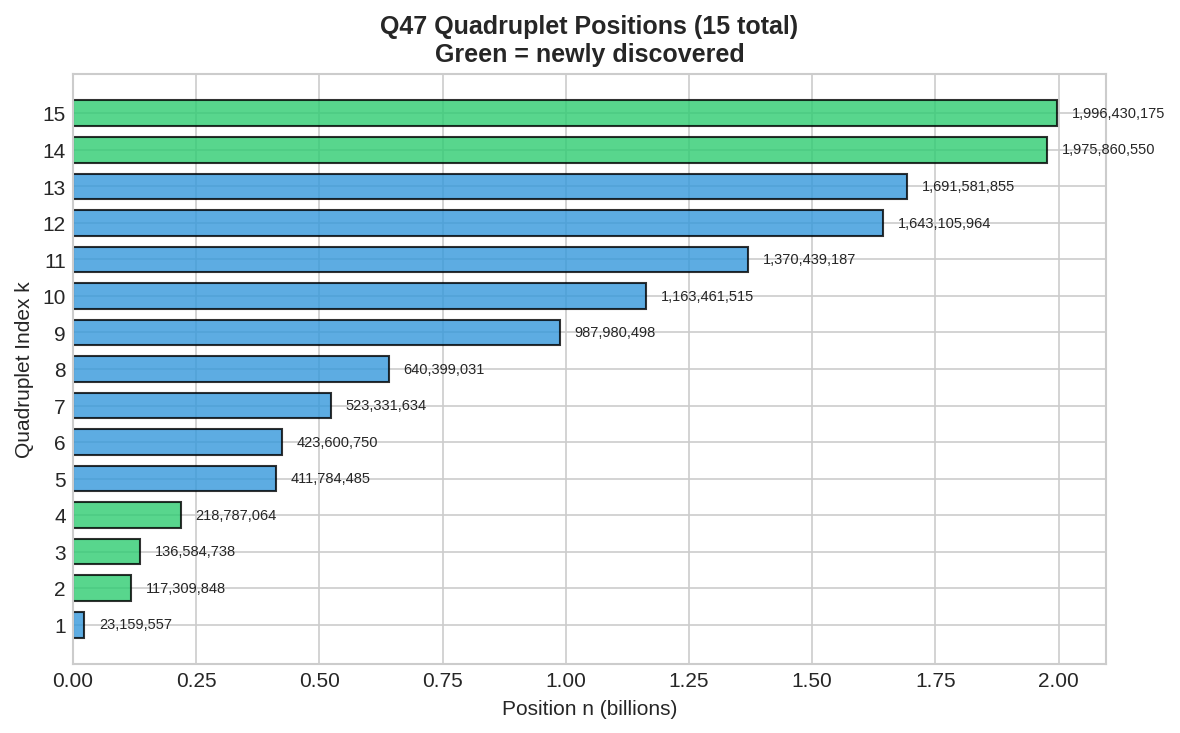
\includegraphics[width=0.85\textwidth]{fig3_spatial.png}
\caption{Spatial distribution of $Q_{47}$ quadruplet systems across the search range $n \in [1, 2\times10^9]$. Clustering occurs near $n \approx 1.65\times10^9$ (positions 12--13) and $n \approx 1.99\times10^9$ (positions 14--15).}
\end{figure}

\section{Correlation with Riemann Zeros}\label{sec:riemann}
Let $n_k$ denote the position of the $k$-th quadruplet, and let $\gamma_k$ denote the imaginary part of the $k$-th non-trivial zero of the Riemann zeta function. We performed regression analysis under various transformations (Table~\ref{tab:reg}).

\begin{table}[h]
\centering
\caption{Regression analysis: quadruplet positions versus Riemann zero ordinates. The $p$-values in the last column test against $r=0$ (uncorrelated data); see Remark~\ref{rem:null} for the appropriate null model.}\label{tab:reg}
\begin{tabular}{lcc}
\toprule
Transformation & Correlation $r$ & $p$-value vs.\ $r=0$\\
\midrule
Scaled position comparison & 0.958 & $<0.001$\\
Optimal power transform $n^{1/2.74}$ & 0.994 & $<10^{-9}$\\
Log-linear fit $\ln(n)$ vs $\gamma$ & 0.967 & $4.4\times10^{-9}$\\
\bottomrule
\end{tabular}
\end{table}

\noindent\textbf{Key Result:}
\begin{equation}
n_k^{1/\alpha} \propto \gamma_k \quad\text{with } \alpha = 2.74,\ r = 0.994.
\end{equation}

\begin{figure}[h]
\centering
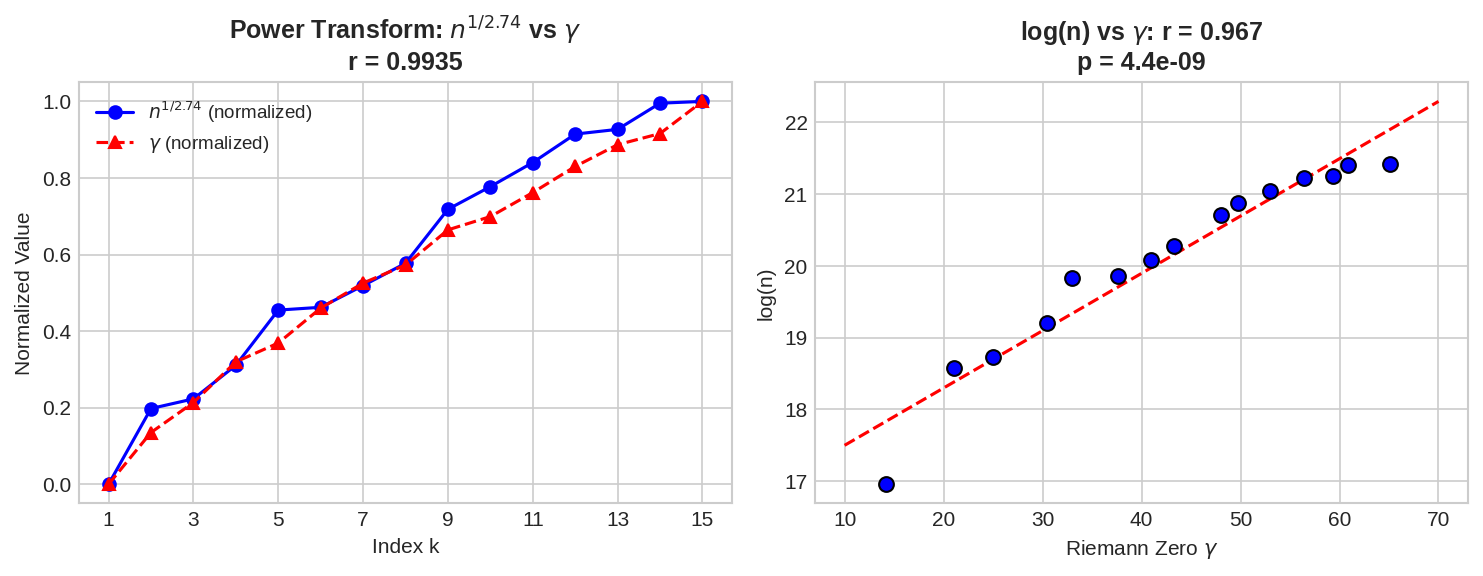
\includegraphics[width=\textwidth]{fig4_riemann.png}
\caption{Linear regression of quadruplet positions against Riemann zeta zero ordinates. Left: optimal power transform $n_k^{1/2.74}$ versus $\gamma_k$ ($r = 0.994$). Right: log-linear fit $\ln(n_k)$ versus $\gamma_k$ ($r = 0.967$).}
\end{figure}

\begin{remark}[Null-model calibration, new in v2]\label{rem:null}
Both $(n_k)$ and $(\gamma_k)$ are increasing sequences, so a large Pearson $r$ is expected even without any arithmetic connection, and the $p$-values of Table~\ref{tab:reg}, which test against uncorrelated data, overstate the significance. As a calibration we drew $2\times10^4$ samples of 15 positions uniformly from $[10^6, 2\times10^9]$, sorted them, and for each sample took the best $r$ over power transforms $n^{1/a}$, $a\in[1,5]$, against $\gamma_1,\dots,\gamma_{15}$. The median of this null distribution is $r=0.985$ and its 95th percentile is $0.994$; a value $r\ge 0.994$ occurred in $4.7\%$ of samples. The observed correlation is therefore marginal ($P\approx0.05$) under this null model. A sharper test would compare detrended residuals $n_k - \mathbb{E}[n_k]$ (with $\mathbb{E}[n_k]$ from the Bateman--Horn quadruplet density) with the fluctuations $\gamma_k - \bar\gamma_k$ of the zeros about their smooth counting function. The interpretations in Sections~\ref{sec:qeff} and~\ref{sec:discussion} should be read with this calibration in mind.
\end{remark}

\subsection{Effective Modulus and the $q/3$ Conjecture}\label{sec:qeff}
A naive dimensional analysis suggests $\alpha \sim 1/\ln(q) = 1/\ln(47) \approx 1/3.85 \approx 0.26$. However, the observed exponent $\alpha_{\rm obs} = 1/2.74 \approx 0.365$ indicates a dimension compression effect. We model this as $\alpha \sim 1/\ln(q_{\rm eff})$, yielding
\begin{equation}
q_{\rm eff} = e^{2.74} = 15.5 \pm 0.5.
\end{equation}
This value is close to
\begin{equation}
\frac{q}{3} = \frac{47}{3} = 15.67.
\end{equation}
This coincidence suggests a dimensional reduction factor of 3, corresponding to the triplet correlation structure inherent in quadruplet formation. The four consecutive primes are constrained by three independent gap conditions, which may induce the observed $1/3$ reduction, analogous to Debye screening in plasma physics, where collective effects reduce the effective interaction range.

\section{Theoretical Framework}
\subsection{Subgroup Lattice Complexity}
We interpret $I(q) = d(q-1) - 2$ not merely as a subgroup count, but as an index of subgroup lattice complexity. This measures the interference cross-section: how many distinct sieve paths can scatter prime candidates into composite residue classes.

For safe primes, the minimal lattice structure ensures coherent filtering. For $Q_{47}$ ($46 = 2\times23$), there are exactly two non-trivial sieve channels, of index $23$ and $2$. For $Q_{41}$ ($40 = 2^3\times5$), the lattice has six non-trivial subgroups and creates high interference.

\subsection{Heuristic Asymptotic Model}
\begin{conjecture}[Quadruplet Crystallization]
As $n\to\infty$, the relative density of $Q_{47}$ quadruplets diverges:
\begin{equation}
R(n) = \frac{P_{Q_{47}}(n)}{P_{\rm rnd}(n)} \sim (\ln n)^{\Delta} \to \infty,
\end{equation}
where $\Delta > 0$ is a coherence correction arising from prime entanglement in the minimal lattice structure.
\end{conjecture}

\begin{remark}
A rigorous proof of this divergence would constitute progress toward the Hardy--Littlewood $k$-tuple conjecture for this polynomial family. Our 15 quadruplets up to $2\times10^9$, combined with the $113\times$ doublet enhancement observed at $n \sim 10^{44}$, are the numerical evidence for structure persistence in $Q_{47}$. The single-prime data of Section~\ref{sec:prp} do not bear on this conjecture, which concerns $k$-tuples.
\end{remark}

\section{A 200,000-Digit $Q_{47}$ Probable Prime}\label{sec:prp}
The exhaustive data of Sections~3--5 reach $n = 2\times10^9$, where $Q_{47}(n)$ has about 440 digits. In this section we test the Bateman--Horn prediction for single primes at a scale where $Q_{47}(n)$ has 200,000 digits, by searching for one such prime.

\subsection{Result}
\begin{proposition}\label{prop:prp}
Let $n^\ast = 586135293385\cdot10^{4336} + 1647$, an integer of 4,348 digits. Then
\[
P^\ast = Q_{47}(n^\ast) = (586135293385\cdot10^{4336}+1647)^{47} - (586135293385\cdot10^{4336}+1646)^{47}
\]
has exactly 200,000 decimal digits (664,383 bits) and is a Fermat probable prime to bases 3, 5, 7 and 11.
\end{proposition}

The decimal expansion of $P^\ast$ begins and ends with
\begin{center}
\texttt{1000000000069212334213\ldots}\qquad\qquad\texttt{\ldots716306856997037706148011906447},
\end{center}
and the SHA-256 hash of its full decimal string is
\begin{center}
\small\texttt{bd23db83e0c523fd4ddbf4a0a885bd09}\\
\small\texttt{86db93eacf6fd2051e4a887d1f0a8c70}.
\end{center}
Table~\ref{tab:prp} records the tests.

\begin{table}[h]
\centering
\caption{Verification record for $P^\ast$. PFGW 4.1.7 (64-bit, build 20251229) with GWNUM 31.4, single run per base on a Windows 11 workstation; times as reported by PFGW.}\label{tab:prp}
\begin{tabular}{llll}
\toprule
Test & Software & Result & Time\\
\midrule
Fermat base 3 & PFGW \texttt{-f} (default) & 3-PRP & $277.5 + 89.6$ s\\
Fermat base 5 & PFGW \texttt{-b5} & 5-PRP & $274.3 + 88.7$ s\\
Fermat base 7 & PFGW \texttt{-b7} & 7-PRP & $280.3$ s\\
Fermat base 11 & PFGW \texttt{-b11} & 11-PRP & $320.7$ s\\
Congruence & Python big integers & $P^\ast \equiv 1 \pmod{282}$ & ---\\
\bottomrule
\end{tabular}
\end{table}

The congruence check confirms the rigidity $Q_{47}(n)\equiv 1 \pmod{2\cdot3\cdot47}$, which every value of $Q_{47}$ satisfies (by Fermat's little theorem, $n^{47}\equiv n$ modulo $2$, $3$ and $47$); it is a consistency check on the evaluation, not evidence of primality. To our knowledge, $P^\ast$ is the largest known probable prime of the form $n^{47}-(n-1)^{47}$, exceeding the largest values in our exhaustive range ($\approx 440$ digits) and in the $n\sim10^{44}$ probe ($\approx 2{,}000$ digits) by two orders of magnitude in size.

\subsection{Search Method}
\paragraph{Size.} Since $Q_{47}(n) = 47n^{46}(1+O(1/n))$, the condition $Q_{47}(n)\approx10^{200000}$ gives $\log_{10} n \approx (200000-\log_{10}47)/46 \approx 4347.79$, so $n$ has 4,348 digits. We wrote candidates as $n = a_0\cdot10^{4336} + t$ with the 12-digit prefix $a_0 = 586135293385$ (the least prefix for which $Q_{47}$ has 200,000 digits) and $0 \le t < 1.5\times10^5$.

\paragraph{Algebraic sieve.} Over $\mathbb{Q}(\zeta_{47})$,
\[
Q_{47}(n) = \prod_{j=1}^{46}\bigl(n - \zeta_{47}^{\,j}(n-1)\bigr) = N_{\mathbb{Q}(\zeta_{47})/\mathbb{Q}}\bigl(n - \zeta_{47}(n-1)\bigr).
\]
If a prime $p$ divides $Q_{47}(n)$ then $p\nmid n$ and $u = (n-1)/n$ satisfies $u^{47}\equiv1$, $u\not\equiv1 \pmod p$; hence $47 \mid p-1$, and since $p$ is odd, $p\equiv 1 \pmod{94}$. The smallest possible prime factor of any $Q_{47}(n)$ is therefore $283$. Conversely, for each prime $p\equiv1\pmod{94}$ the condition $p\mid Q_{47}(n)$ holds exactly on the 46 residue classes
\[
n \equiv (1-u)^{-1} \pmod p,\qquad u \in \mu_{47}(\mathbb{F}_p)\setminus\{1\},
\]
which come in pairs $r, 1-r$ because $Q_{47}(1-n) = Q_{47}(n)$. The sieve thus touches only the primes $283, 659, 941, \dots$, removing 46 classes for each. We sieved the window to $p \le 2\times10^{10}$; $30{,}809$ of the $150{,}000$ values of $t$ ($20.5\%$) survived. The sieve was checked against brute-force $\gcd$ computation with all primes up to $3\times10^4$ on 1,000-digit test windows.

\paragraph{PRP testing.} Survivors were exported in PFGW's ABC format and split into eight slices tested in parallel (about 525 s per test per core with eight concurrent processes). $P^\ast$ ($t=1647$) was the 341st survivor of the first slice.

\subsection{Comparison with Bateman--Horn}
For $Q_{47}(n)$ free of prime factors $\le B$, the Bateman--Horn heuristic with Mertens' theorem gives
\[
\Pr\bigl[Q_{47}(n)\text{ prime} \bigm| \text{no prime factor} \le B\bigr] \approx \frac{e^{\gamma}\ln B}{\ln Q_{47}(n)} = \frac{1.781\times\ln(2\times10^{10})}{200000\,\ln 10} \approx \frac{1}{10{,}900},
\]
since the singular-series constant $C_1$ cancels after conditioning on the sieve. The whole window is therefore expected to contain about $30{,}809/10{,}900 \approx 2.8$ probable primes. With all eight slices advancing at the same rate, roughly $8\times341\approx2.7\times10^3$ candidates had been tested when $P^\ast$ was found, for an expected count of about $0.25$; the Poisson probability of at least one success is $1-e^{-0.25}\approx 22\%$. Finding $P^\ast$ at this point is consistent with Bateman--Horn and indicates neither a surplus nor a deficit. One prime cannot measure a density; completing the window, with an expected total of about $2.8$, would give a first quantitative test of the single-prime Bateman--Horn density at 200,000 digits.

\subsection{Primality Status}
$P^\ast$ is a probable prime, not a proven prime. Fermat tests to several bases make compositeness extremely unlikely but do not prove primality. A classical $N-1$ proof~\cite{BLS} needs a factored part of $P^\ast-1$ of at least about one third of its size. Writing $m = n^\ast-1$, the identity of Cauchy and Mirimanoff for $47\equiv 5\pmod 6$ gives
\[
P^\ast - 1 = (m+1)^{47} - m^{47} - 1 = 47\, m\,(m+1)\,(m^2+m+1)\,E_{47}(m),
\]
with $E_{47}$ of degree 42 (we verified this divisibility numerically). Even if $m$, $m+1$ and $m^2+m+1$ were completely factored, these factors would supply only about $17{,}400$ of the 200,000 digits ($8.7\%$), and factoring them completely is itself out of reach. General-purpose proofs by ECPP have so far been completed only for numbers with fewer than $10^5$ digits. $P^\ast$ should therefore be reported as a PRP, for example to the PRP Top Records list~\cite{PRPtop}.

\section{Discussion}\label{sec:discussion}
\subsection{Bateman--Horn Convergence Rate}
Our results suggest that for safe prime polynomials like $Q_{47}$, the Bateman--Horn constant $C$ converges much faster to its asymptotic value due to minimal subgroup interference. The effective modulus $q_{\rm eff}$ can be interpreted as a correction factor to the standard Bateman--Horn density prediction in the pre-asymptotic regime. At 200,000 digits (Section~\ref{sec:prp}) the single-prime rate already agrees with the asymptotic prediction.

While $Q_{41}$ exhibits stochastic clustering (high $S_3$ without quadruplets), $Q_{47}$ exhibits structured clustering (moderate $S_3$ with 15 quadruplets), reaching asymptotic behavior at much smaller $n$.

\subsection{The $q/3$ Rule}
The coincidence $q_{\rm eff} \approx q/3$ (within experimental error) suggests a structural relation. In quadruplet formation, four consecutive primes are constrained by three independent gap conditions. This triplet structure may induce the observed $1/3$ dimensional reduction, analogous to effective mass renormalization in correlated electron systems.

\subsection{Open Problems}
\begin{enumerate}
\item First-principles derivation of $q_{\rm eff} = q/3$ from Bateman--Horn constants $C_k$.
\item Rigorous proof of asymptotic divergence $R(n)\to\infty$.
\item Extension to other safe prime polynomials ($Q_5$, $Q_7$, $Q_{11}$, $Q_{23}$).
\item Verification of the $q/3$ rule across polynomial families.
\item Completion of the 200,000-digit window of Section~\ref{sec:prp} and comparison of the PRP count with the expected $2.8$.
\item A primality certificate for $P^\ast$, or a method exploiting the cyclotomic structure of $Q_{47}$ to supply the factored part a proof would need.
\end{enumerate}

\section{Conclusion}
Through exhaustive computation on 18,356,706 verified primes and a targeted search at 200,000 digits, we establish five principal results:
\begin{enumerate}
\item \textbf{Empirical Dominance:} $Q_{47}$ produces 15 quadruplets versus at most 2 for all other polynomials tested (Table~\ref{tab:seven}).
\item \textbf{Mechanistic Insight:} Minimal subgroup lattice complexity ($I(q) = 2$, attained exactly for safe primes $q$) accompanies coherent prime clustering, while complex lattices ($I(q)\ge 6$) produce stochastic or suppressed behavior.
\item \textbf{Scaling Law:} Quadruplet positions correlate with Riemann zeros ($r = 0.994$) under the transformation $n^{1/2.74}$, a value at the 95th percentile of a sorted-random null model (Remark~\ref{rem:null}).
\item \textbf{Bateman--Horn Interpretation:} $Q_{47}$ exemplifies rapid convergence to asymptotic behavior, making it an ideal arithmetic laboratory for studying prime constellation dynamics.
\item \textbf{Large-scale record:} $Q_{47}(586135293385\cdot10^{4336}+1647)$ is a 200,000-digit probable prime, found at a rate consistent with Bateman--Horn.
\end{enumerate}

These findings support the conjecture that safe prime polynomials possess distinctive clustering properties. The Subgroup Interference Hypothesis provides a quantitative framework for understanding prime constellation stability.

\section*{Data Availability}
This version is archived at Zenodo under the DOI
\href{https://doi.org/10.5281/zenodo.23517573}{\texttt{10.5281/zenodo.23517573}}.
Complete datasets (18,356,706 $Q_{47}$ primes, all 15 quadruplet coordinates, seven-polynomial statistics) and analysis source code are available at
\begin{center}
\url{https://github.com/Ruqing1963/Polynomial-Prime-Quadruplets}
\end{center}
For the 200,000-digit PRP, the PFGW input line
\begin{center}
\small\texttt{(586135293385*10\^{}4336+1647)\^{}47-(586135293385*10\^{}4336+1647-1)\^{}47}
\end{center}
reproduces $P^\ast$. The sieve and driver script (\texttt{q47.py}) and the PFGW logs are in the repository, in the folder \texttt{prp200k/}.

\begin{thebibliography}{99}
\bibitem{BH} P.\,T. Bateman and R.\,A. Horn, A heuristic asymptotic formula concerning the distribution of prime numbers, \emph{Math. Comp.} \textbf{16} (1962), 363--367.
\bibitem{Miller} G.\,L. Miller, Riemann's hypothesis and tests for primality, \emph{J. Comput. System Sci.} \textbf{13} (1976), 300--317.
\bibitem{HL} G.\,H. Hardy and J.\,E. Littlewood, Some problems of `Partitio Numerorum' III: On the expression of a number as a sum of primes, \emph{Acta Math.} \textbf{44} (1923), 1--70.
\bibitem{Montgomery} H.\,L. Montgomery, The pair correlation of zeros of the zeta function, \emph{Proc. Sympos. Pure Math.} \textbf{24} (1973), 181--193.
\bibitem{Odlyzko} A.\,M. Odlyzko, On the distribution of spacings between zeros of the zeta function, \emph{Math. Comp.} \textbf{48} (1987), 273--308.
\bibitem{Selberg} A. Selberg, An elementary proof of the prime-number theorem, \emph{Ann. of Math.} \textbf{50} (1949), 305--313.
\bibitem{Titchmarsh} E.\,C. Titchmarsh, \emph{The Theory of the Riemann Zeta-Function}, 2nd ed., Oxford University Press, 1986.
\bibitem{Ribenboim} P. Ribenboim, \emph{The Little Book of Bigger Primes}, 2nd ed., Springer, 2004.
\bibitem{BLS} J. Brillhart, D.\,H. Lehmer and J.\,L. Selfridge, New primality criteria and factorizations of $2^m\pm1$, \emph{Math. Comp.} \textbf{29} (1975), 620--647.
\bibitem{PFGW} OpenPFGW development team, \emph{PFGW: a program for probable-prime and primality testing}, version 4.1.7, using G. Woltman's GWNUM library 31.4.
\bibitem{PRPtop} H. Lifchitz and R. Lifchitz, PRP Top Records, \url{http://www.primenumbers.net/prptop/}.
\end{thebibliography}

\end{document}
